% vim: set textwidth=78 autoindent:

\section{Creating PyQGIS Applications}

% when the revision of a section has been finalized, 
% comment out the following line:
% \updatedisclaimer

One of the goals of QGIS is to provide not only an application, but a set of
libraries that can be used to create new applications. This goal has been
realized with the refactoring of libraries that took place after the release
of 0.8. Since the release of 0.9, development of standalone applications using
either C++ or Python is possible. We recommend you use QGIS 1.0.0 or greater
as the basis for your python applications because since this version we now
provide a stable consistent API.

In this chapter we'll take a brief look at the process of creating a
standalone Python application. The QGIS blog has several examples for creating
PyQGIS\footnote{An application created using Python and the QGIS bindings}
applications. We'll use one of them as a starting point to get a look at how
to create an application.

The features we want in the application are:

\begin{itemize}
\item Load a vector layer
\item Pan
\item Zoom in and out
\item Zoom to the full extent of the layer
\item Set custom colors when the layer is loaded
\end{itemize} 

This is a pretty minimal feature set. Let's start by designing the GUI using
Qt Designer. 

\subsection{Designing the GUI}

Since we are creating a minimalistic application, we'll take the same
approach with the GUI. Using Qt Designer, we create a simple MainWindow with
no menu or toolbars. This gives us a blank slate to work with. To create the
MainWindow:

\begin{enumerate}
\item Create a directory for developing the application and change to it
\item Run Qt Designer
\item The \qtdialog{New Form} dialog should appear. If it doesn't, choose
\qtdropmenuopt{New Form...} from the \qtmainmenuopt{File} menu.
\item Choose \qtdropmenuopt{Main Window} from 
the \qtdropmenuopt{templates/forms} list
\item Click \qtdropmenuopt{Create} 
\item Resize the new window to something manageable
\item Find the \qtdropmenuopt{Frame} widget in the list 
(under \qtdropmenuopt{Containers}) and drag it to
the main window you just created
\item Click outside the frame to select the main window area 
\item Click on the \qtdropmenuopt{Lay Out in a Grid} tool. When you do, the frame
will expand to fill your entire main window
\item Save the form as \usertext{mainwindow.ui} 
\item \qtdropmenuopt{Exit} Qt Designer
\end{enumerate} 

Now compile the form using the PyQt interface compiler:

\begin{verbatim}
   pyuic4 -o mainwindow_ui.py mainwindow.ui
\end{verbatim}

This creates the Python source for the main window GUI. Next we need to create
the application code to fill the blank slate with some tools we can use.

\subsection{Creating the MainWindow}

Now we are ready to write the \classname{MainWindow} class that will do the real work.
Since it takes up quite a few lines, we'll look at it in chunks, starting
with the import section and environment setup:

\begin{verbatim}
1 # Loosely based on:
2 #   Original C++ Tutorial 2 by Tim Sutton
3 #   ported to Python by Martin Dobias
4 #   with enhancements by Gary Sherman for FOSS4G2007
5 # Licensed under the terms of GNU GPL 2
6
7 from PyQt4.QtCore import *
8 from PyQt4.QtGui import *
9 from qgis.core import *
10 from qgis.gui import *
11 import sys
12 import os
13 # Import our GUI
14 from mainwindow_ui import Ui_MainWindow
15 
16 # Environment variable QGISHOME must be set to the 1.0 install directory
17 # before running this application
18 qgis_prefix = os.getenv("QGISHOME")
\end{verbatim}

Some of this should look familiar from our plugin, especially the PyQt4 and
QGIS imports. Some specific things to note are the import of our GUI in line
14 and the import of our CORE library on line 9.

Our application needs to know where to find the QGIS installation. Because
of this, we set the \usertext{QGISHOME} environment variable to point to the 
install directory of QGIS 1.x In line 20 we store this value from
the environment for later use.

Next we need to create our \classname{MainWindow} class which will contain
all the logic of our application.
\begin{verbatim}
21 class MainWindow(QMainWindow, Ui_MainWindow):
22 
23   def __init__(self):
24     QMainWindow.__init__(self)
25 
26     # Required by Qt4 to initialize the UI
27     self.setupUi(self)
28 
29     # Set the title for the app
30     self.setWindowTitle("QGIS Demo App")
31 
32     # Create the map canvas
33     self.canvas = QgsMapCanvas()
34     # Set the background color to light blue something
35     self.canvas.setCanvasColor(QColor(200,200,255))
36     self.canvas.enableAntiAliasing(True)
37     self.canvas.useQImageToRender(False)
38     self.canvas.show()
39 
40     # Lay our widgets out in the main window using a 
41     # vertical box layout
42     self.layout = QVBoxLayout(self.frame)
43     self.layout.addWidget(self.canvas)
44 
45     # Create the actions for our tools and connect each to the appropriate
46     # method
47     self.actionAddLayer = QAction(QIcon("(qgis_prefix + "/share/qgis/themes/classic/mActionAddLayer.png"),
48     \
49         "Add Layer", self.frame)
50     self.connect(self.actionAddLayer, SIGNAL("activated()"), self.addLayer)
51     self.actionZoomIn = QAction(QIcon("(qgis_prefix + "/share/qgis/themes/classic/mActionZoomIn.png"), \
52         "Zoom In", self.frame)
53     self.connect(self.actionZoomIn, SIGNAL("activated()"), self.zoomIn)
54     self.actionZoomOut = QAction(QIcon("(qgis_prefix + "/share/qgis/themes/classic/mActionZoomOut.png"), \
55         "Zoom Out", self.frame)
56     self.connect(self.actionZoomOut, SIGNAL("activated()"), self.zoomOut)
57     self.actionPan = QAction(QIcon("(qgis_prefix + "/share/qgis/themes/classic/mActionPan.png"), \
58         "Pan", self.frame)
59     self.connect(self.actionPan, SIGNAL("activated()"), self.pan)
60     self.actionZoomFull = QAction(QIcon("(qgis_prefix + "/share/qgis/themes/classic/mActionZoomFullExtent.png"), \
61         "Zoom Full Extent", self.frame)
62     self.connect(self.actionZoomFull, SIGNAL("activated()"),
63     self.zoomFull)
64 
65     # Create a toolbar
66     self.toolbar = self.addToolBar("Map")
67     # Add the actions to the toolbar
68     self.toolbar.addAction(self.actionAddLayer)
69     self.toolbar.addAction(self.actionZoomIn)
70     self.toolbar.addAction(self.actionZoomOut);
71     self.toolbar.addAction(self.actionPan);
72     self.toolbar.addAction(self.actionZoomFull);
73 
74     # Create the map tools
75     self.toolPan = QgsMapToolPan(self.canvas)
76     self.toolZoomIn = QgsMapToolZoom(self.canvas, False) # false = in
77     self.toolZoomOut = QgsMapToolZoom(self.canvas, True) # true = out
\end{verbatim}

Lines 21 through 27 are the basic declaration and initialization of the 
\classname{MainWindow} and the set up of the user interface using the 
\method{setupUi} method. This is required for all applications.

Next we set the title for the application so it says something more
interesting than \usertext{MainWindow} (line 30). Once that is
complete, we are ready to complete the user interface. When we created it in
Designer, we left it very sparse---just a main window and a frame. You could
have added a menu and the toolbar using Designer, however we'll do it with
Python.

In lines 33 through 38 we set up the map canvas, set the background color to a
light blue, and enable antialiasing.  We also tell it not to use a
\classname{QImage} for rendering (trust me on this one) and then set the
canvas to visible by calling the \method{show} method.

Next we set the layer to use a vertical box layout within the frame and add
the map canvas to it in line 43.

Lines 48 to 63 set up the actions and connections for the tools in our
toolbar. For each tool, we create a \classname{QAction} using the icon we
defined in the QGIS classic theme.  Then we connect up the
\usertext{activated} signal from the tool to the method in our class that will
handle the action. This is similar to how we set things up in the plugin
example.

Once we have the actions and connections, we need to add them to the toolbar.
In lines 66 through 72 we create the toolbar and add each tool to it.

Lastly we create the three map tools for the application (lines 75 through
77). We'll use the map tools in a moment when we define the methods to make
our application functional. Let's look at the methods for the map tools.

\begin{verbatim}
78   # Set the map tool to zoom in
79   def zoomIn(self):
80     self.canvas.setMapTool(self.toolZoomIn)
81 
82   # Set the map tool to zoom out
83   def zoomOut(self):
84     self.canvas.setMapTool(self.toolZoomOut)
85 
86   # Set the map tool to 
87   def pan(self):
88    self.canvas.setMapTool(self.toolPan)
89 
90   # Zoom to full extent of layer
91   def zoomFull(self):
92     self.canvas.zoomFullExtent()
\end{verbatim}

For each map tool, we need a method that corresponds to the connection we made
for each action. In lines 79 through 88 we set up a method for each of the
  three tools that interact with the map. When a tool is activated by clicking
  on it in the toolbar, the corresponding method is called that ``tells'' the
  map canvas it is the active tool. The active tool governs what happens when
  the mouse is clicked on the canvas.

The \usertext{zoom to full extent} tool isn't a map tool---it does its job
without requiring a click on the map. When it is activated, we call the
\method{zoomFullExtent} method of the map canvas (line 92).  This completes
the implementation of all our tools except one---the \usertext{Add Layer}
tool. %FIXME 
Let's look at it next:

\begin{verbatim}
93   # Add an OGR layer to the map
94   def addLayer(self):
95     file = QFileDialog.getOpenFileName(self, "Open Shapefile", ".", "Shapefiles
96     (*.shp)")
97     fileInfo = QFileInfo(file)
98 
99     # Add the layer
100     layer = QgsVectorLayer(file, fileInfo.fileName(), "ogr")
101
102    if not layer.isValid():
103      return
104
105    # Change the color of the layer to gray
106    symbols = layer.renderer().symbols()
107    symbol = symbols[0]
108    symbol.setFillColor(QColor.fromRgb(192,192,192))
109
110    # Add layer to the registry
111    QgsMapLayerRegistry.instance().addMapLayer(layer);
112
113    # Set extent to the extent of our layer
114    self.canvas.setExtent(layer.extent())
115
116    # Set up the map canvas layer set
117    cl = QgsMapCanvasLayer(layer)
118    layers = [cl]
119    self.canvas.setLayerSet(layers)
\end{verbatim}

In the \method{addLayer} method we use a \classname{QFileDialog} to get the
name of the shapefile to load. This is done in line 96.
Notice that we specify a ``filter'' so the dialog will only show files of
type \filename{.shp}.

Next in line 97 we create a \classname{QFileInfo} object from the shapefile
path.  Now the layer is ready to be created in line 100. Using the
\classname{QFileInfo} object to get the file name from the path we specify it 
for the name of the layer when it is created.  To make sure that the layer is 
valid and won't cause any problems when loading, we check it in line 102. If
it's bad, we bail out and don't add it to the map canvas.

Normally layers are added with a random color. Here we want to tweak the
colors for the layer to make a more pleasing display. Plus we know we are
going to add the \filename{world\_borders} layer to the map and this will make
it look nice on our blue background. To change the color, we need to get the
symbol used for rendering and use it to set a new fill color. This is done in
lines 106 through 108. 

All that's left is to actually add the layer to the registry and a few other
housekeeping items (lines 111 through 119). This stuff is standard for adding
a layer and the end result is the world borders on a light blue background.
The only thing you may not want to do is set the extent to the layer, if you
are going to be adding more than one layer in your application.

That's the heart of the application and completes the \classname{MainWindow} class. 

\subsection{Finishing Up}

The remainder of the code shown below creates the \object{QgsApplication}
object, sets the path to the QGIS install, sets up the \method{main} method
and then starts the application. The only other thing to note is that we move
the application window to the upper left of the display. We could get fancy
and use the Qt API to center it on the screen.

\begin{verbatim}
120 def main(argv):
121   # create Qt application
122   app = QApplication(argv)
123 
124   # Initialize qgis libraries
125   QgsApplication.setPrefixPath(qgis_prefix, True)
126   QgsApplication.initQgis()
127 
128   # create main window
129   wnd = MainWindow()
130   # Move the app window to upper left
131   wnd.move(100,100)
132   wnd.show()
133 
134   # run!
135   retval = app.exec_()
136   
137   # exit
138   QgsApplication.exitQgis()
139   sys.exit(retval)
140 
141 
142 if __name__ == "__main__":
143   main(sys.argv)
\end{verbatim}

\subsection{Running the Application}

Now we can run the application and see what happens. Of course if you are like 
most developers, you've been testing it out as you went along. 

Before we can run the application, we need to set some environment variables. 

\nix{}\osx{}
\begin{verbatim}
export LD_LIBRARY_PATH=$HOME/qgis/lib%$
export PYTHONPATH=$HOME/qgis/share/qgis/python
export QGISHOME=$HOME/qgis%$
\end{verbatim}

\win{}
\begin{verbatim}
set PATH=C:\qgis;%PATH%
set PYTHONPATH=C:\qgis\python
set QGISHOME=C:\qgis
\end{verbatim}

We assume
\begin{itemize}
\item\nix{}\osx{}QGIS is installed in 
your home directory in 
\filename{qgis}. 
\item\win{}QGIS is installed in \filename{C:\textbackslash qgis}.
\end{itemize}

When the application starts up, it looks like this:

\begin{figure}[ht]
\begin{center}
  \caption{Starting the new demo application \nixcaption} \label{fig:demo_app_startup}
  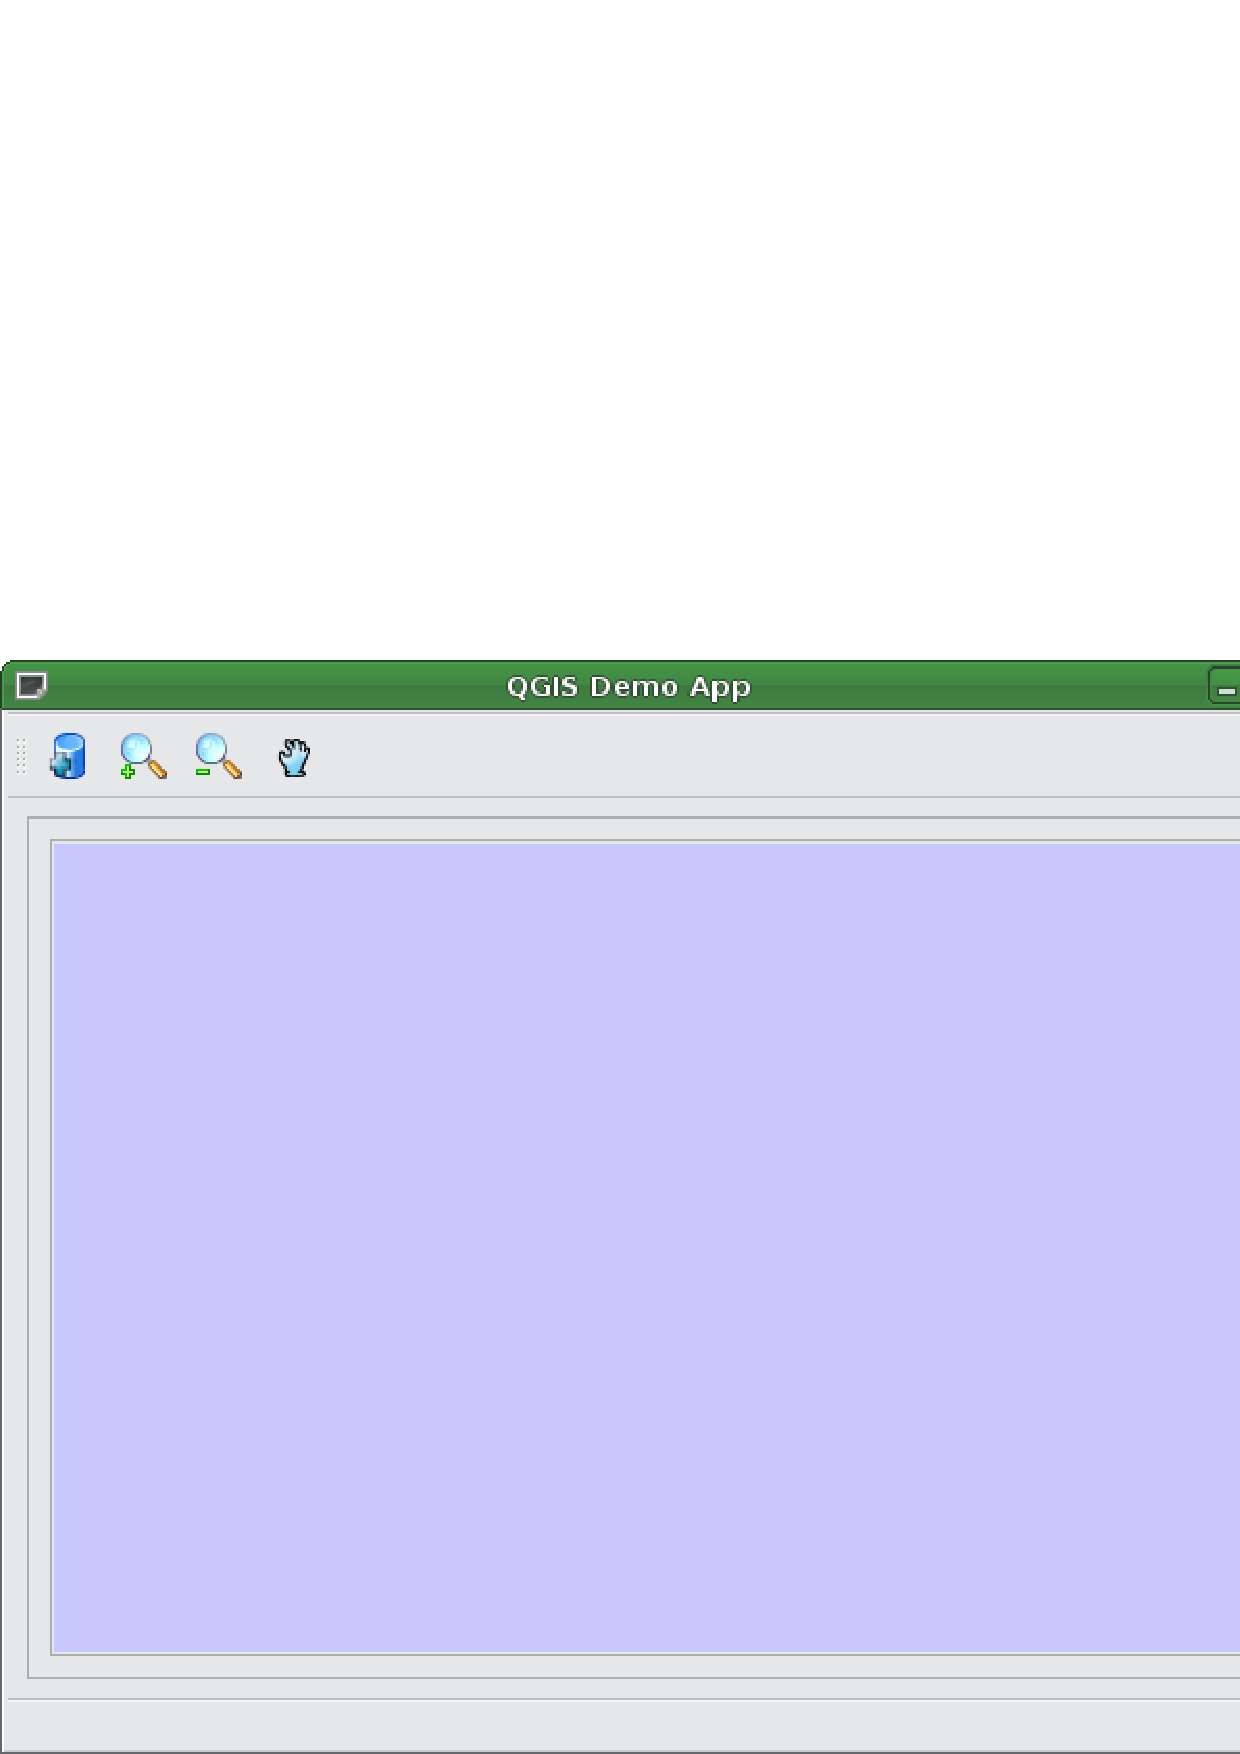
\includegraphics[clip=true, width=12cm]{python1_application}
\end{center}
\end{figure}

To add the \filename{world\_borders} layer, click on the 
\usertext{Add Layer} tool and navigate to the data directory.
Select the shapefile and click \button{Open} to add it to the map. 
Our custom fill color is applied and the result is shown in Figure \ref{fig:demo_app_done}.

Creating a PyQGIS application is really pretty simple.  In less than 150 lines
of code we have an application that can load a shapefile and navigate the map.
If you play around with the map, you'll notice that some of the built-in
features of the canvas also work, including mouse wheel scrolling and panning
by holding down the \keystroke{Space} bar and moving the mouse.

Some sophisticated applications have been created with PyQGIS and more are in 
the works. This is pretty impressive, considering that this development has 
taken place even before the official release of QGIS 1.0.

\begin{figure}[ht]
\begin{center}
  \caption{Adding a layer the demo application \nixcaption} \label{fig:demo_app_done}
  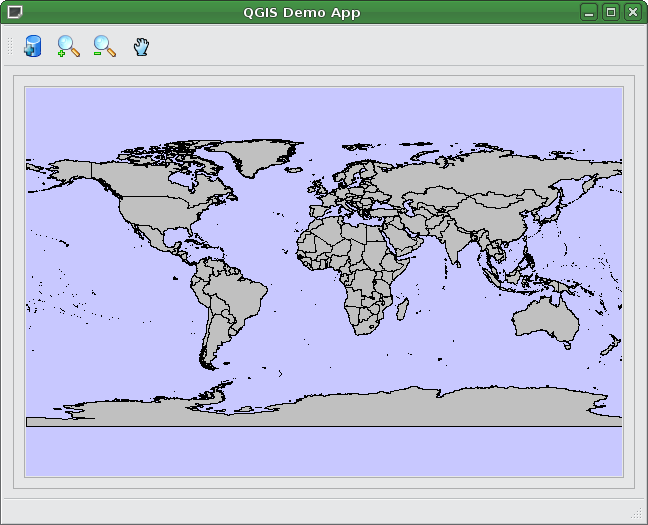
\includegraphics[clip=true, width=12cm]{python2_application}
\end{center}
\end{figure}

